\documentclass[10pt,a4paper,twocolumn,twoside]{article}

% ------------------------------------------------------------------ packages
\usepackage[T1]{fontenc}
\usepackage{lmodern}
\usepackage[a4paper,margin=2cm,columnsep=7mm]{geometry}
\usepackage{amsmath,amssymb}
\usepackage{siunitx}
\usepackage{booktabs}
\usepackage{tabularx}
\usepackage{graphicx}
\usepackage[font=small,labelfont=bf]{caption}
\usepackage{parskip} % new paragraphs start flush left, with a blank line between them
\usepackage{url}
\usepackage{microtype}
\usepackage[numbers,sort&compress]{natbib}
\usepackage[hidelinks]{hyperref}
\usepackage[capitalise,noabbrev]{cleveref}

\graphicspath{{../figures/}{figures/}}
\setlength{\emergencystretch}{1.5em} % fewer overfull lines in narrow columns

% ------------------------------------------------------------------ layout
\raggedbottom % even spacing between paragraphs and headings (no stretching to fill columns)
% let floats use more of a page, so tables and figures stay close to their text
\renewcommand{\topfraction}{0.85}
\renewcommand{\bottomfraction}{0.5}
\renewcommand{\textfraction}{0.15}
\renewcommand{\floatpagefraction}{0.75}
\renewcommand{\dbltopfraction}{0.85}
\renewcommand{\dblfloatpagefraction}{0.75}
\setcounter{topnumber}{3}
\setcounter{dbltopnumber}{3}

% ------------------------------------------------------------------ notation
\newcommand{\Hs}{H_{s}}
\newcommand{\Tp}{T_{p}}
\newcommand{\pct}[1]{#1\,\%}
\newcommand{\vect}[1]{\boldsymbol{#1}}
\DeclareMathOperator*{\argmin}{arg\,min}
\DeclareMathOperator*{\argmax}{arg\,max}

\title{Reading the sea from vessel motion:\\
       sea state estimation from heave and pitch using CIM-ML thinking}
\author{William Boland \quad Olve Grønås Birkeland\\[2pt]
        \small TMR06 Autonomous Systems, NTNU}
\date{}

\begin{document}

% Title and abstract span both columns
\makeatletter
\twocolumn[
\begin{@twocolumnfalse}
\maketitle
\begin{abstract}
\noindent
The motions of a vessel on dynamic positioning (DP) carry information about the sea state around
it. This paper compares three ways of estimating the significant wave height $\Hs$ and the peak
period $\Tp$ from measured heave and pitch: a physics-based inversion through the motion response
amplitude operators (RAOs), data-driven regression on the log motion spectra by partial least
squares (PLS) and principal component regression (PCR), and a hybrid based on Harald Martens'
hybrid modelling framework, in which PLS corrects the physics estimate. The methods are tested on
250 co-simulations of RV Gunnerus in the Open Simulation Platform (OSP), in head, long-crested
JONSWAP seas. The inversion uses a different RAO set from the one in the simulator, so the physics
method has a realistic model error. On 50 hidden test runs the hybrid gave the lowest error,
\pct{1.94} in $\Hs$ and \pct{0.74} in $\Tp$, against \pct{5.81} and \pct{0.95} for the physics
fit. PLS alone was better than the physics in $\Hs$ and worse in $\Tp$. A robustness study shows
that the gain depends on the RAO error and sensor noise seen in training. A small frequency shift
of the true RAOs brings the hybrid back to about the accuracy of the physics fit, and a change in
sensor noise makes PLS fail, while the physics fit is barely affected.
\end{abstract}
\vspace{1.5em}
\end{@twocolumnfalse}
]
\makeatother

% ==================================================================
\section{Introduction}
\label{sec:intro}
% ==================================================================

A ship responds to the waves around it, and its motions can be measured cheaply and continuously
with an inertial measurement unit. Using the vessel itself as a wave sensor, the \emph{wave buoy
analogy}, therefore gives on-site sea state information for decision support, operability
assessment and DP control \citep{nielsen2017,brodtkorb2018}.

The difficulty is that the ship acts as a filter. How much it moves depends on the wave frequency
and direction, as described by its RAOs, so the accuracy of the estimate depends on how well the
RAOs are known. Model-based methods invert the motion spectra through the RAOs, either directly or
by fitting a wave spectrum \citep{tannuri2003}. \citet{nielsen2017} reviews these techniques, and
\citet{brodtkorb2018} apply them to a vessel on DP. They need no training data, but they inherit
every error in the RAOs, which change with loading and are never known exactly.

Data-driven regression takes the opposite route. It learns the link from motions to sea state
directly and needs no RAOs, but it needs training data with a known sea state and may not work
outside them. A hybrid model keeps the physics as the base and uses the data only to correct its
systematic error. The hybrid in this paper is built on the framework of \citet{martens2023}, which
has three steps. Known causal structure is modelled first, from theory (deduction). Small
data-driven models, such as principal component analysis (PCA) and partial least squares (PLS),
then find the variation that is left (induction). Finally a person interprets what was found
(abduction). Here the physics inversion is the deductive step and PLS the inductive step;
\cref{sec:theory_hybrid} sets out where the hybrid follows the framework and where it departs from
it. Martens also argues that small, interpretable models use less energy and are easier to trust
than large neural networks \citep{martens2025}, which matters for an estimator running on board a
vessel.

A pitfall when such methods are tested on simulated data is the \emph{inverse crime}
\citep{kaipio2005}: if the same model generates and inverts the data, there is no model error, and
the inversion looks far better than it would on a real vessel.

This paper asks two questions. First, how accurately can $\Hs$ and $\Tp$ be estimated from 20
minutes of heave and pitch on a DP vessel in head seas, and does a hybrid of physics and PLS help?
Second, how much of any gain remains when the vessel or the sensor differs from the one the models
were trained on? The data are simulated, so the true sea state is known, and the inverse crime is
avoided by inverting with a different RAO set from the one the simulator uses. \Cref{sec:method}
describes the methods and the case study, \cref{sec:results} the results, and
\cref{sec:conclusion} the conclusions.

% ==================================================================
\section{Method}
\label{sec:method}
% ==================================================================

\subsection{Waves and vessel response}
\label{sec:theory_waves}

In linear wave theory an irregular, long-crested sea is a sum of regular waves with random phases
\citep{faltinsen1990}. It is described by the wave spectrum $S_\zeta(\omega)$, which shows how the
wave energy is spread over frequency. The two quantities estimated here are the significant wave
height and the peak period,
\begin{equation}
\begin{gathered}
\Hs = 4\sqrt{m_0}, \qquad \Tp = 2\pi/\omega_p, \\
m_0 = \int_0^\infty S_\zeta\,d\omega, \qquad \omega_p = \argmax_\omega S_\zeta(\omega),
\end{gathered}
\label{eq:hs_tp}
\end{equation}
where $m_0$ is the area under the spectrum and $\omega_p$ the frequency of its peak.

A common model for a wind sea is the JONSWAP spectrum \citep{dnv2021c205}: the
Pierson--Moskowitz spectrum of a fully developed sea, with a sharper peak.
\begin{align}
S_J(\omega) &= A_\gamma\, S_{\mathrm{PM}}(\omega)\, \gamma^{\,r(\omega)}, \label{eq:jonswap}\\
S_{\mathrm{PM}}(\omega) &= \tfrac{5}{16}\,\Hs^2\,\omega_p^4\,\omega^{-5}
\exp\!\left[-\tfrac{5}{4}\left(\omega_p/\omega\right)^4\right], \nonumber\\
r(\omega) &= \exp\!\left[-\frac{(\omega-\omega_p)^2}{2\sigma^2\omega_p^2}\right]. \nonumber
\end{align}
The remaining symbols only shape the peak:

\begin{center}\small
\begin{tabularx}{\columnwidth}{@{}l >{\raggedright\arraybackslash}X l@{}}
\toprule
Symbol & Role & Value \\
\midrule
$\gamma$ & Peak enhancement: how much higher and sharper the peak is than in $S_{\mathrm{PM}}$ ($\gamma=1$ gives $S_{\mathrm{PM}}$) & 3.3 \\
\addlinespace[4pt]
$\sigma$ & Width of the enhanced peak, below / above $\omega_p$ & 0.07 / 0.09 \\
\addlinespace[4pt]
$A_\gamma$ & Normalisation that keeps the area close to $\Hs^2/16$ & $1-0.287\ln\gamma$ \\
\bottomrule
\end{tabularx}
\end{center}

$\Hs$ appears only in $S_{\mathrm{PM}}$, as the factor $\Hs^2$. The spectrum is therefore the wave
height squared times a shape $s$ that depends only on $\Tp$ and $\gamma$,
\begin{equation}
S_J(\omega; \Hs, \Tp, \gamma) = \Hs^2\, s(\omega; \Tp, \gamma).
\label{eq:hs_scaling}
\end{equation}
This property is used throughout the paper.

For small motions the vessel responds linearly to the waves. Its response in degree of freedom $j$
to a regular wave of unit amplitude, frequency $\omega$ and heading $\beta$ relative to the bow is
given by the RAO $H_j(\omega,\beta)$ \citep{faltinsen1990}. The motion spectrum is then the wave
spectrum filtered by the RAO,
\begin{equation}
S_{x_j}(\omega) = |H_j(\omega, \beta)|^2\, S_\zeta(\omega).
\label{eq:response}
\end{equation}
A DP vessel in head seas makes this simpler in three ways. The vessel holds its position, so it
meets the waves at their own frequency. The hull is symmetric, so roll is zero in head seas and
only heave and pitch carry information. And the DP system only counteracts slow motion in surge,
sway and yaw, so it does not affect the wave-frequency heave and pitch \citep{fossen2021}.

\subsection{Estimating the motion spectra}
\label{sec:theory_welch}

The motion spectra are estimated from the measured records with Welch's method
\citep{welch1967}: the record is cut into overlapping, windowed segments, and the spectra of the
segments are averaged. Three things about this estimate matter below. First, each segment of length $T_{\mathrm{seg}}$
gives one spectrum with frequency resolution $\Delta f = 1/T_{\mathrm{seg}}$. Long segments
resolve the peak finely, but a record of fixed length then holds fewer of them, so less averaging is
possible and the estimate is noisier. Second, the random error of the estimate is proportional to the spectrum itself, so the methods
below work with the logarithm of the spectrum. Third, the window smears the true spectrum slightly over
neighbouring frequencies, described by a kernel $K$. Sensor noise with standard deviation
$\sigma_n$, sampled every $\Delta t$, adds a flat floor $N = 2\sigma_n^2\Delta t$. The expected
estimate is therefore
\begin{equation}
\operatorname{E}\big[\hat S_x(f)\big] = \big(K * S_x\big)(f) + N.
\label{eq:welch}
\end{equation}

\subsection{Physics inversion}
\label{sec:theory_inverse}

\paragraph{Spectral division.}
The simplest inversion divides the measured motion spectrum by the squared RAO,
\begin{equation}
\begin{gathered}
\hat S_\zeta(f) = \frac{\hat S_x(f)}{|H(f)|^2},
\\
f \in \{ f : |H(f)| > c \max |H| \},
\end{gathered}
\label{eq:division}
\end{equation}
and then computes $\Hs$ and $\Tp$ from \cref{eq:hs_tp}. Where the RAO is small, the division
amplifies noise and RAO errors, so only frequencies where $|H|$ is above a share $c = 0.2$ of its
maximum are used. Two limits follow: wave energy outside this band is missed, and $\Tp$ can only
take the values $1/f_k$ of the frequency bins.

\paragraph{JONSWAP fit.}
The fit avoids both limits by assuming that the wave spectrum has the JONSWAP shape. It searches
for the $\Hs$, $\Tp$ and $\gamma$ whose \emph{predicted} motion spectra best match the measured
ones. The prediction includes the same effects as the measurement in \cref{eq:welch}, the window
smearing and the noise floor:
\begin{equation}
\begin{gathered}
M_j(f; \vect\theta) = \big( K * \big[ |H_j|^2\, S_J \big] \big)(f) + N_j, \\
S_J = S_J(\cdot\,; \Hs, \Tp, \gamma), \qquad \vect\theta = (\ln\Hs, \ln\Tp, \ln\gamma).
\end{gathered}
\label{eq:model}
\end{equation}
The parameters minimise the squared difference in log scale, summed over the motions used and over
the same frequencies as in the division:
\begin{equation}
\begin{split}
\hat{\vect\theta} &= \argmin_{\vect\theta} \sum_j \sum_{f} \varepsilon_j(f; \vect\theta)^2, \\
\varepsilon_j(f; \vect\theta) &= \ln M_j(f; \vect\theta) - \ln \hat S_{x_j}(f).
\end{split}
\label{eq:fit}
\end{equation}
Working in log scale suits the error of the estimate and gives the low-energy parts of the spectrum
a fair weight. Including the smearing $K$ avoids a bias in $\Tp$ for narrow peaks. Including the
noise floor keeps the model from dropping far below the measurement where the motion is weak.

\paragraph{What the motion spectra cannot tell.}
By \cref{eq:response,eq:hs_scaling}, the motion spectrum is $S_{x_j} = |H_j|^2\,\Hs^2\,s(\omega;\Tp,\gamma)$.
A vessel whose RAOs are all $g$ times larger therefore gives exactly the same motion spectra as the
original vessel in waves $g$ times higher, and no method that only sees the motion spectra can tell
the two apart. An error in the overall RAO level goes straight into $\Hs$ and leaves $\Tp$
unchanged, since $\Tp$ depends only on where the energy lies in frequency. This is why a physics
inversion usually estimates $\Tp$ well and $\Hs$ less well. An error in the \emph{shape} of the
RAO, such as a shift of the natural frequencies with loading, changes the motion spectra in a way no
sea state can copy exactly, so it can in principle be detected.

\subsection{Data-driven regression}
\label{sec:theory_regression}

The data-driven models take as input the log spectra of heave and pitch over the analysed band,
stacked into one vector $\vect x$ per record, and predict $\vect y = (\ln\Hs, \ln\Tp)$. The inputs
are centred and scaled to unit variance on the training runs. The logarithm follows from
\cref{eq:response,eq:hs_scaling}:
\begin{equation}
\begin{split}
\log_{10} S_{x_j}(f) &= 2\log_{10}\Hs + \log_{10}|H_j(f)|^2 \\
&\quad + \log_{10} s(f; \Tp, \gamma).
\end{split}
\label{eq:log_linear}
\end{equation}
In log scale, $\Hs$ adds the same constant to every frequency bin, so a linear model can recover it
easily. $\Tp$ instead moves the shape $s$ along the frequency axis, which is not linear in the
inputs, so it needs more components. With log targets the squared error is also a relative error.
\citet{martens2023} uses the same step: the logarithm turns products of known and unknown factors
into sums, which linear models handle well.

Neighbouring frequency bins move together, so the inputs are strongly correlated and ordinary least
squares would be unstable. Both methods therefore first compress the inputs into a few components
and regress on those \citep{hastie2009}. Principal component regression (PCR) uses the directions
of largest variance in the inputs, which are chosen without looking at the targets. Partial least
squares (PLS) chooses each component to covary as much as possible with the targets
\citep{wold2001}, so it usually needs fewer. The number of components $A$ is chosen by
cross-validation.

\subsection{Hybrid model}
\label{sec:theory_hybrid}

Following \citet{martens2023}, the hybrid keeps the physics estimate and lets the data correct it:
\begin{equation}
\begin{split}
\ln \hat{\vect y} &= \ln \hat{\vect y}_{\text{phys}} + \hat{\vect r}(\vect x),
\\
\vect r &= \ln\vect y - \ln\vect y_{\text{phys}},
\end{split}
\label{eq:hybrid}
\end{equation}
where $\hat{\vect r}$ is a PLS model from the log spectra to the error of the physics fit to heave
and pitch. With no components, the correction is just the average error of the physics. With more,
it can depend on the shape of the spectrum, for example on how much energy lies where the RAOs are
wrong. The physics already handles the hard part (the position of the peak and the $\Hs^2$
scaling), so PLS only has to learn a smooth correction. This should need fewer components and less
data than learning everything from the spectra.

\paragraph{Relation to Martens' framework.}
The hybrid follows the order of \citet{martens2023}: known physics first, data only for what is
left. It also shares the log transform and the use of a small PLS model chosen by
cross-validation. It departs from the framework in three ways. Martens removes the known structure
from the measurements and models the residual spectra; here PLS maps the full spectra to the error
of the target estimate. Martens uses PCA on the residuals to look for unknown structure; here the
residuals are not examined. And the step where a person interprets the components before they are
trusted is left out. \Cref{sec:robustness} shows what this costs.

\subsection{Validation}
\label{sec:theory_validation}

Each method is scored on $n$ runs by the root-mean-square (RMS) relative error and by the bias,
the mean relative error:
\begin{equation}
\begin{gathered}
e_i = \frac{\hat y_i}{y_i} - 1, \\
\mathrm{RMS} = \sqrt{\frac{1}{n}\sum_{i=1}^{n} e_i^2}, \qquad
\mathrm{bias} = \frac{1}{n}\sum_{i=1}^{n} e_i.
\end{gathered}
\label{eq:scores}
\end{equation}
The number of components is chosen by 5-fold
cross-validation on the calibration runs, repeated with three different splits. Every
$A = 0,\dots,40$ is tried, and the one with the lowest sum of $\Hs$ and $\Tp$ error is kept
\citep{hastie2009}. This error is slightly
optimistic, since it was used to make the choice. A separate set of test runs is therefore kept
aside and scored only once, with a 95\,\% bootstrap interval from 2000 resamples of the runs
\citep{hastie2009}.

\subsection{Case study}
\label{sec:case}

The data come from the OSP co-simulation of RV Gunnerus (length overall \SI{36.25}{m})
\citep{ospdpsimpy}. It couples models of the waves, the vessel, the DP controller, an observer and
the thrusters. The waves follow \cref{sec:theory_waves}, and the wave-frequency motion of the vessel
follows \cref{eq:response}, with the slow motion and the DP loop added on top. The conditions are
kept simple, to judge the methods before anything else complicates them: head seas, long-crested
JONSWAP waves with $\gamma = 3.3$, and no wind or current.

There are 250 runs, each with its own sea state. The sea states are spread evenly over
$\Hs = 0.5$--4.0\,m and $\Tp = 4$--14\,s by Latin hypercube sampling, with a steepness limit of
1/15 to keep them realistic. Of these, 200 runs are used for calibration, and 50 runs, drawn with
another sampling seed, are kept aside as test runs. Each run gives 20 minutes of heave and pitch, sampled
every \SI{0.5}{s}, to which white noise is added to represent the motion sensor: \SI{0.02}{m} in
heave and $0.02^\circ$ in pitch, an assumed level.

The spectra use \SI{128}{s} Hann segments with 75\,\% overlap, so $\Delta f \approx \SI{0.008}{Hz}$.
They are kept between 0.04 and 0.4\,Hz, which gives 46 frequency bins per motion and 92 inputs to
the data-driven models. \Cref{fig:spectra} shows typical motion spectra and the noise floor. The code is available online \citep{boland2026sse}.

The inversion uses the RAOs in \path{GunnerusL35_20201112.mat}, while the simulator uses those in
\path{gunnerus.mat}. Both describe RV Gunnerus, but they come from separate calculations and differ
mostly for periods below about \SI{8}{s}. This gives the physics method a realistic model error and
avoids the inverse crime. Five physics estimates are made: spectral division
(\cref{eq:division}) of the heave or the pitch spectrum, and the JONSWAP fit (\cref{eq:fit}) to
heave, to pitch, or to both. The fit to both motions is called \emph{the physics fit} below, and is
the base of the hybrid.

\paragraph{Assumptions.}
The methods and the case study rest on the following assumptions:
\begin{itemize}
\item The waves and the vessel response are linear (\cref{eq:response}).
\item The sea is long-crested, comes from ahead and has a single-peaked JONSWAP spectrum with a
known, fixed $\gamma = 3.3$.
\item The vessel holds position on DP, so it meets the waves at their own frequency, and the DP
system does not affect heave and pitch at wave frequency.
\item The sea state is constant over each 20-minute record.
\item The sensor noise is white, with a known standard deviation that the physics fit uses for
its noise floor.
\item The RAOs used for the inversion are the only source of model error. There is no wind or
current.
\end{itemize}

\begin{figure}[tb]
  \centering
  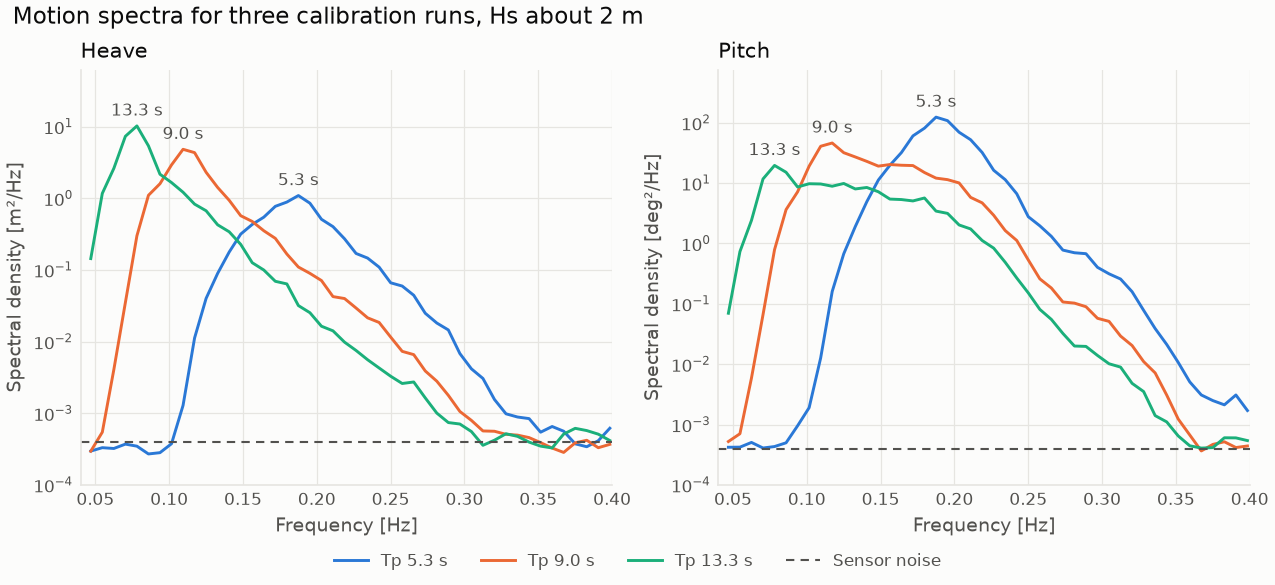
\includegraphics[width=\columnwidth]{spectra.png}
  \caption{Heave and pitch spectra of three calibration runs with $\Hs \approx \SI{2}{m}$, from
           short to long waves, and the sensor noise level.}
  \label{fig:spectra}
\end{figure}

\paragraph{Robustness test.}
The calibration and test runs share the same RAO error and noise level. On a real vessel the RAOs
change with loading, and the sensor may differ from the one assumed. To test this, the models
trained on the calibration runs are kept fixed, and the 50 test sea states are run again with a
changed vessel or sensor:
\begin{itemize}
\item \emph{Gain}: the true heave and pitch RAOs multiplied by $g \in \{0.90, 0.95, 1.05, 1.10\}$.
By \cref{sec:theory_inverse} this should be undetectable.
\item \emph{Frequency shift}: $|H'(\omega)| = |H(\omega/s)|$ with $s \in \{0.95, 0.97, 1.03, 1.05\}$,
a stand-in for a loading change that moves the natural periods by 3--5\,\%.
\item \emph{Sensor noise}: $\sigma_n \in \{0, 0.05, 0.10\}$ (m, deg) instead of 0.02.
\end{itemize}
Each condition uses the same sea states, wave phases and noise draws, so any change in error comes
from the change alone.

% ==================================================================
\section{Results and discussion}
\label{sec:results}
% ==================================================================

\subsection{Physics inversion}

\begin{table}[tb]
  \centering
  \caption{Which physics estimate to start from. RMS relative error and bias [\%] of the five
           physics estimates on the 50 test runs. None of them is fitted to data. The fit to both
           motions is the physics fit, the base of the hybrid.}
  \label{tab:physics}
  \small
  \setlength{\tabcolsep}{4pt}
  \begin{tabular}{@{}ll rr @{\hspace{1.2em}} rr@{}}
    \toprule
    & & \multicolumn{2}{c}{$\Hs$ error} & \multicolumn{2}{c@{}}{$\Tp$ error} \\
    \cmidrule(r{0.9em}){3-4}\cmidrule(l){5-6}
    Method & Motion & RMS & bias & RMS & bias \\
    \midrule
    Division    & Heave &  5.38 &  $+1.30$ & 3.75 & $-1.22$ \\
                & Pitch &  9.62 &  $-8.65$ & 3.47 & $-0.06$ \\
    \addlinespace
    JONSWAP fit & Heave & 22.28 & $+14.75$ & 1.89 & $-1.69$ \\
                & Pitch &  4.79 &  $-4.28$ & 1.02 & $-0.02$ \\
                & \textbf{Both} & \textbf{5.81} & $+2.71$ & \textbf{0.95} & $-0.67$ \\
    \bottomrule
  \end{tabular}
\end{table}

\Cref{tab:physics} answers two questions: which physics estimate the hybrid should start from,
and where its error comes from. The JONSWAP fit estimates $\Tp$ to within 1--2\,\%, against about
3.5\,\% for division, which can only return the period of a frequency bin. Fitting both motions
gives the best $\Tp$. The $\Hs$ errors are larger and biased: estimates from pitch are too low, and
estimates from heave too high. The fit to pitch alone has a slightly lower $\Hs$ error than the fit
to both, but a larger $\Tp$ error. The fit to both is used as the physics fit, since it uses all
the data and has the best $\Tp$, and its $\Hs$ bias is what the correction is meant to remove.
When the simulator's own RAOs are used for the inversion, the $\Hs$ error of the physics fit drops
from about 6\,\% to 1.5\,\%, so almost all of the physics error comes from the RAO mismatch.

The biases follow from the differences between the two RAO files. The pitch RAO used in the
inversion is about 7\,\% too high between 0.08 and 0.2\,Hz, so division from pitch gives an $\Hs$
that is too low by about the same amount. The heave RAO used in the inversion has a dip around
0.2\,Hz, where the measured heave can only be explained by larger waves. This is where short seas
have their peak, so the physics error is largest for $\Tp$ below \SI{6}{s} (\cref{fig:test}).

\subsection{Cross-validation}

\Cref{fig:cv} shows the cross-validated error against the number of components. With no
components, PLS and PCR can only predict the average sea state. The hybrid is then the physics fit
with its average error removed, and is already better than the physics fit alone. PLS reaches its
lowest error at 7 components. PCR needs 25 and improves slowly, since its components are chosen
without looking at the targets. The hybrid needs only 4, which supports the idea that it only has
to learn a smooth correction.

\begin{figure}[tb]
  \centering
  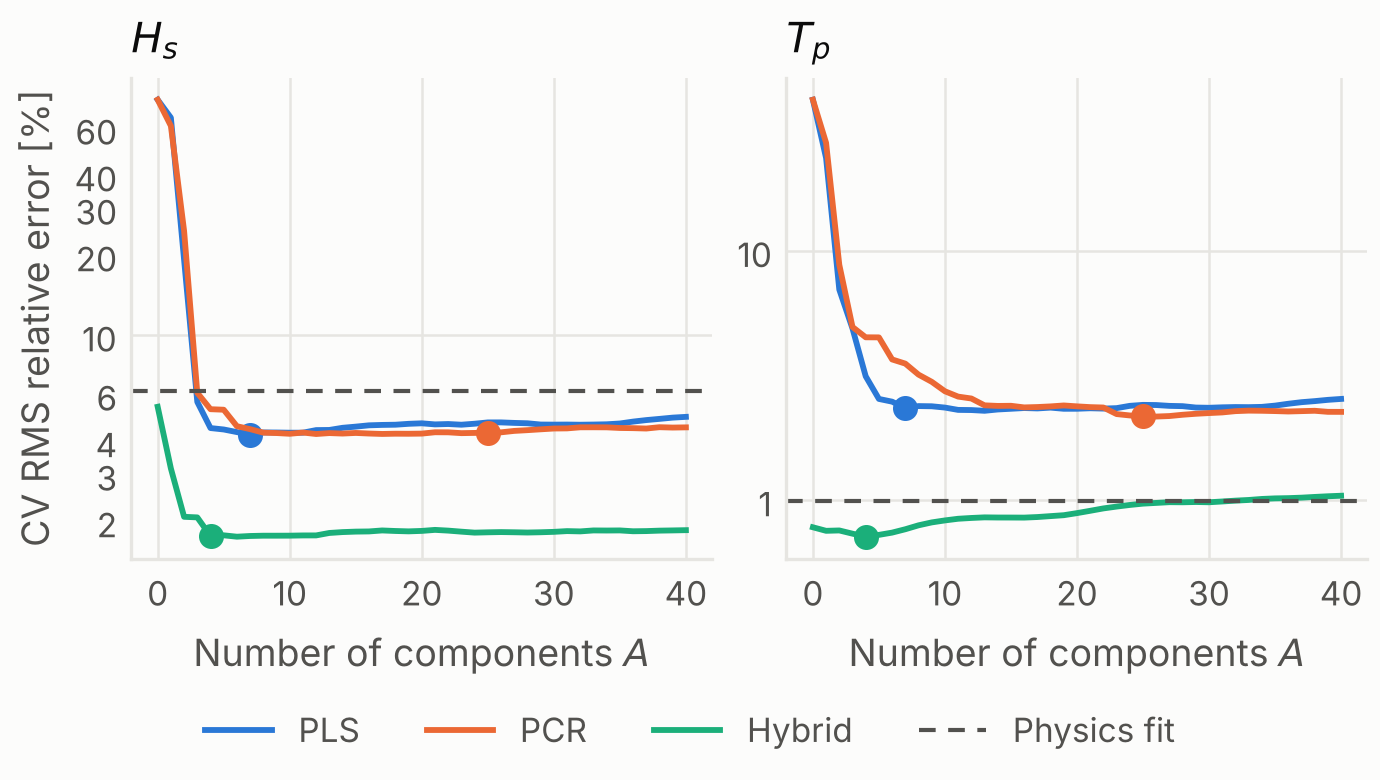
\includegraphics[width=\columnwidth]{cv.png}
  \caption{Cross-validated error against the number of components. Dots mark the chosen number;
           the dashed line is the physics fit, which has no components.}
  \label{fig:cv}
\end{figure}

\subsection{Test runs}

\begin{table}[tb]
  \centering
  \caption{The final methods on the 50 hidden test runs [\%]: RMS relative error with its 95\,\%
           bootstrap interval, and the bias. $A$ is the number of components chosen by
           cross-validation.}
  \label{tab:test}
  \footnotesize
  \setlength{\tabcolsep}{2.2pt}
  \begin{tabular}{@{}l r rcr @{\hspace{0.8em}} rcr@{}}
    \toprule
    & & \multicolumn{3}{c}{$\Hs$ error} & \multicolumn{3}{c@{}}{$\Tp$ error} \\
    \cmidrule(r{0.6em}){3-5}\cmidrule(l){6-8}
    Method & $A$ & RMS & interval & bias & RMS & interval & bias \\
    \midrule
    Physics fit     & --  & 5.81 & 3.99--7.44 & $+2.71$ & 0.95 & 0.78--1.13 & $-0.67$ \\
    PLS             &  7  & 4.25 & 3.23--5.22 & $+0.30$ & 2.12 & 1.72--2.51 & $-0.20$ \\
    PCR             & 25  & 3.96 & 3.01--4.84 & $+0.35$ & 2.12 & 1.72--2.50 & $-0.13$ \\
    \textbf{Hybrid} &  4  & \textbf{1.94} & 1.34--2.50 & $-0.11$ & \textbf{0.74} & 0.57--0.91 & $-0.04$ \\
    \bottomrule
  \end{tabular}
\end{table}

\Cref{tab:test} gives the single evaluation on the test runs. For every method, the
cross-validated error on the calibration runs (\cref{fig:cv}) lies inside the 95\,\% interval of the
test error, so the choices made on the calibration runs did not overfit. The hybrid has the lowest error in both $\Hs$ and $\Tp$, and its $\Hs$
interval lies below those of all other methods. In $\Tp$ it is close to the physics fit, and PLS
and PCR perform about the same. \Cref{fig:test} shows where the gain comes from: the physics fit
overestimates $\Hs$ by up to 19\,\% in short seas, and the correction removes most of this, while it
changes little for longer waves, where the physics is already close.

\begin{figure}[tb]
  \centering
  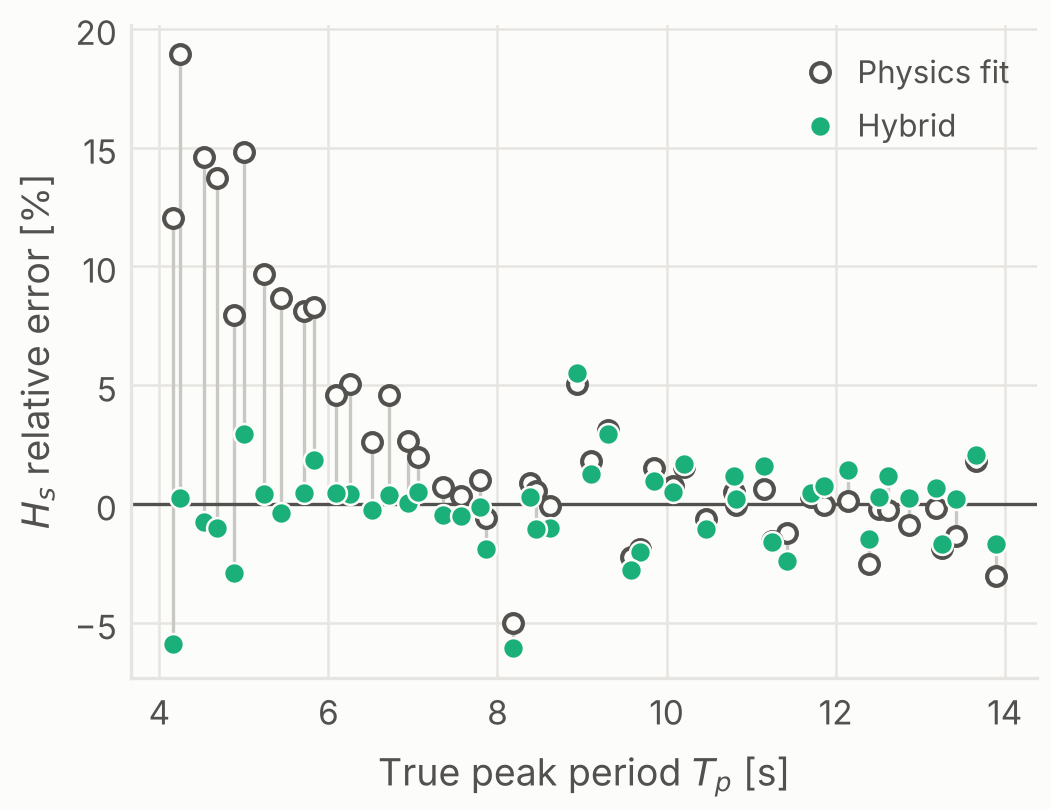
\includegraphics[width=\columnwidth]{test.png}
  \caption{$\Hs$ error of each test run before (physics fit) and after (hybrid) the PLS
           correction, against the true $\Tp$. A grey line joins the two estimates of one run.}
  \label{fig:test}
\end{figure}

\begin{figure*}[t]
  \centering
  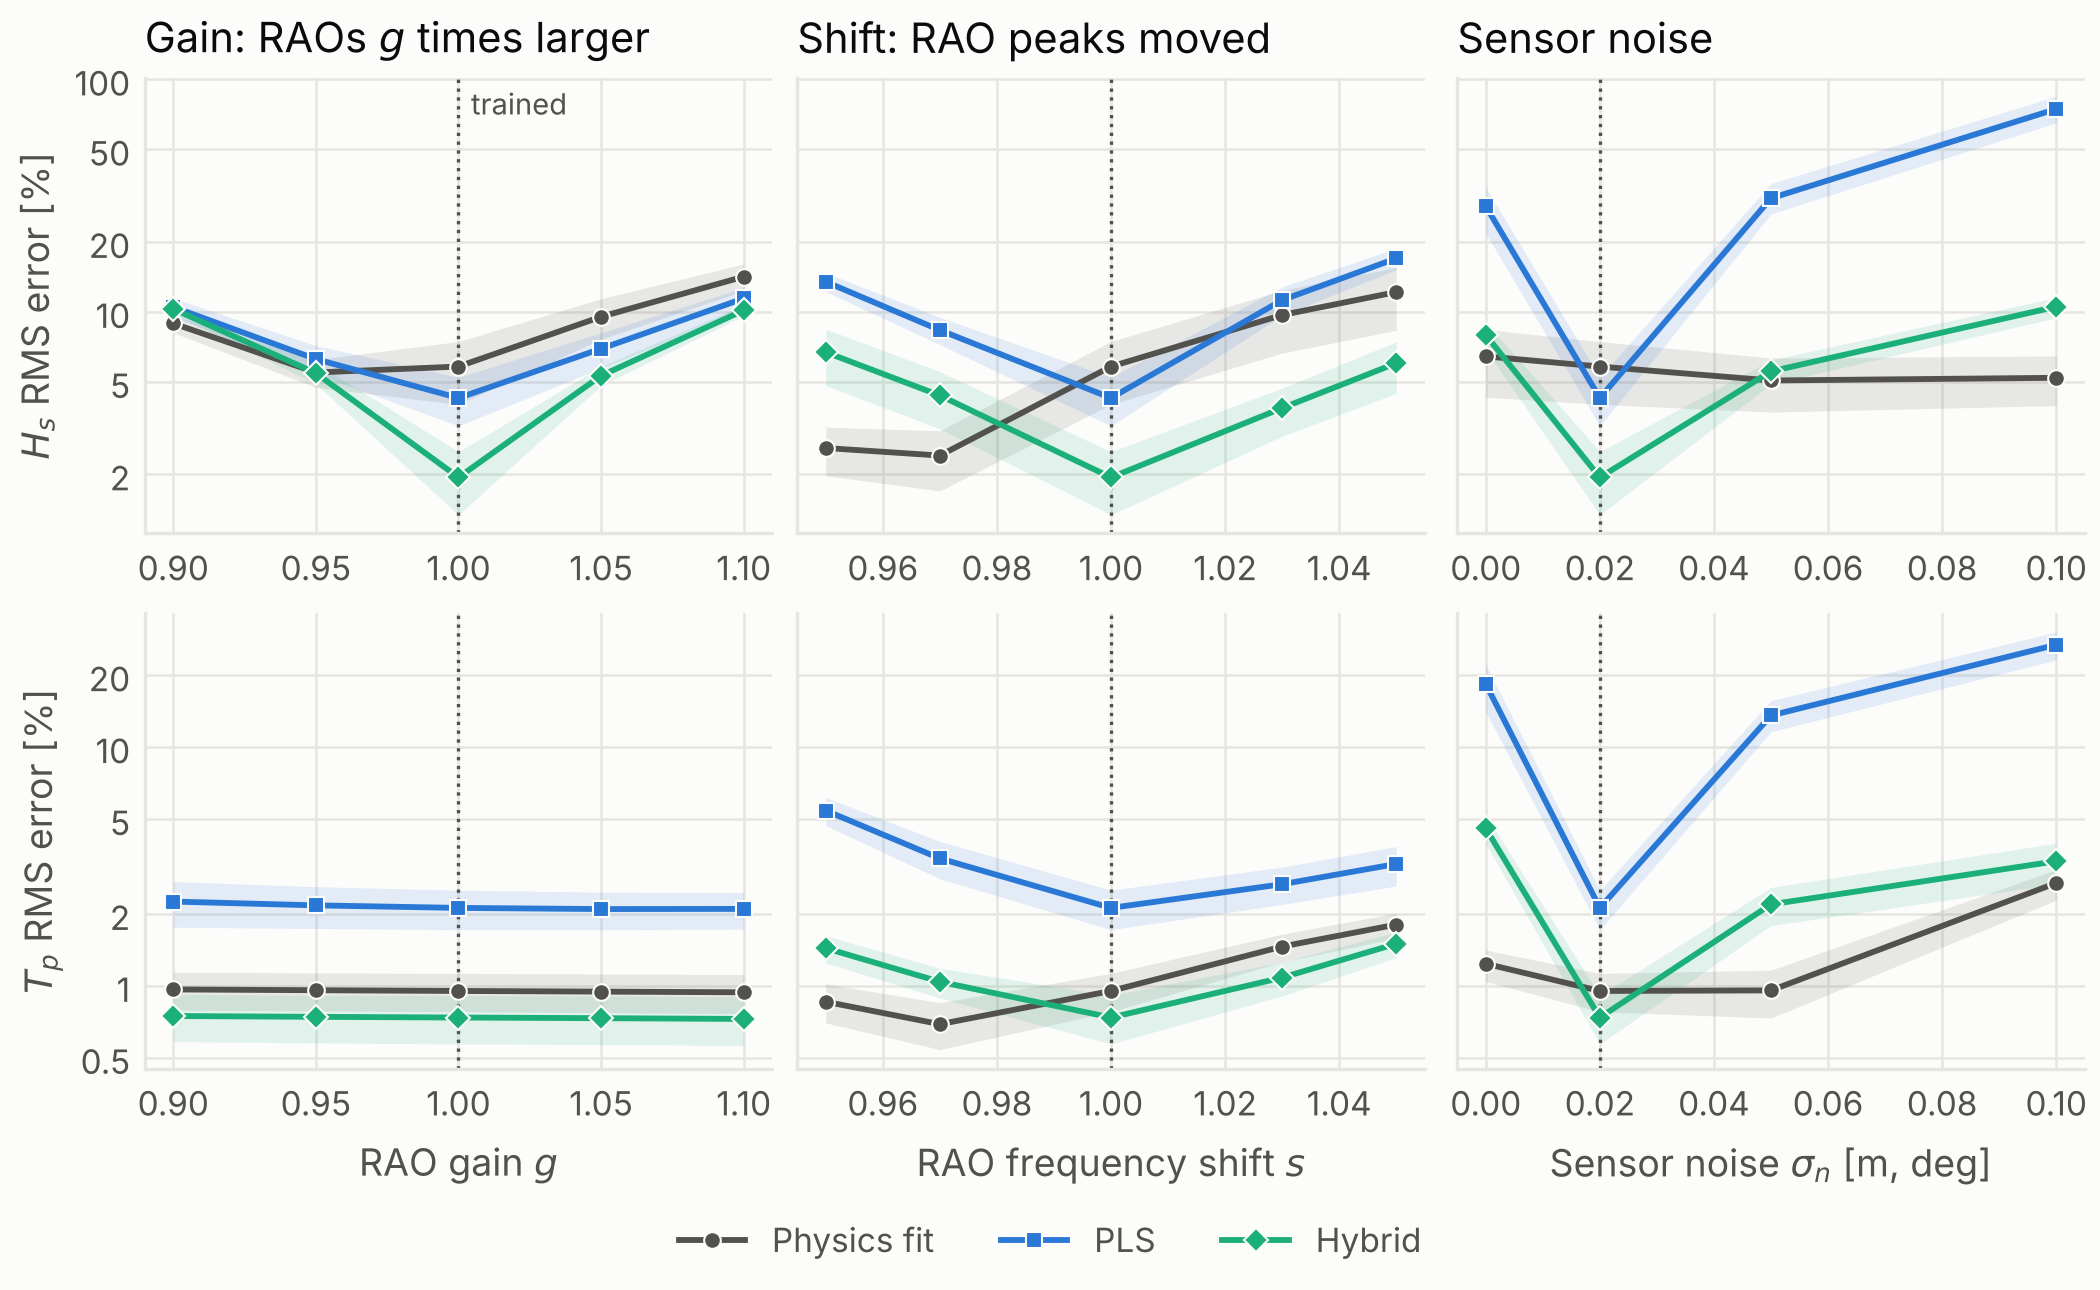
\includegraphics[width=\textwidth]{robust.png}
  \caption{Test-run RMS error of the fixed models when the true vessel (gain, shift) or the sensor
           (noise) differs from training, with 95\,\% bootstrap intervals. The dotted line marks
           the condition the models were trained on. Each row has one logarithmic scale.}
  \label{fig:robust}
\end{figure*}

The results match the theory in \cref{sec:method}. The physics fit finds the spectral peak
precisely, so $\Tp$ is good, but any error in the RAO level goes straight into $\Hs$. PLS has the
opposite profile: $\Hs$ is a single linear direction in the log spectra (\cref{eq:log_linear}),
while $\Tp$ needs several components to follow the peak along the frequency axis. The hybrid keeps
the $\Tp$ accuracy of the physics and removes most of its $\Hs$ error with four PLS components,
coming close to the physics fit with the correct RAOs. This is the division of labour
\citet{martens2023} argues for: the physics carries the known structure, and the data only learn
what is left.

\subsection{Robustness to an unseen vessel or sensor}
\label{sec:robustness}

\Cref{fig:robust} shows the errors of the fixed models when the true vessel or the sensor changes.
The unchanged control gives \cref{tab:test} again.

\paragraph{Gain.}
As predicted in \cref{sec:theory_inverse}, a common RAO gain shifts the $\Hs$ estimate of every
method by about the same factor and leaves $\Tp$ unchanged. A gain of 0.90 or 1.10 gives the hybrid
a bias of about 10\,\% in $\Hs$. The absolute level of the RAOs must therefore come from outside the
motion data, for example a model test or a comparison with a wave buoy.

\paragraph{Frequency shift.}
This is the more realistic case, since loading moves the natural periods. A shift of 3--5\,\% takes
away most of the hybrid's gain, and its $\Hs$ error rises to about the level of the physics fit.
PLS degrades most, since it has learned where the spectral features of one particular vessel lie.
The physics fit improves for shifts below 1, which partly cancel the mismatch between the RAO
files, and gets worse above 1. Over all four shifts the hybrid still has the smallest worst-case
error. Its correction has learned one specific RAO error and loses most of its value when that
error changes. In Martens' framework the residual spectra would be examined before the correction
is trusted. A frequency shift leaves a pattern around the RAO peaks that no sea state can explain
(\cref{sec:theory_inverse}), but the hybrid never looks at the residual spectra, so nothing in it
signals that the vessel has changed.

\paragraph{Sensor noise.}
The physics fits hardly change in $\Hs$, since they only use frequencies where the RAO is large and
the motion stands well above the noise. Their $\Tp$ error grows at the highest noise level. PLS
fails: its $\Hs$ error reaches \pct{74} at the highest noise level, and its bias changes sign with
the noise level. About a third of the heave bins and a sixth of the pitch bins lie within a factor
of three of the noise floor (\cref{fig:spectra}). In log scale these bins weigh as much as the
peak, so PLS has learned the noise floor as part of the wave signal. The hybrid inherits this in a
weaker form. A data-driven model on log spectra must therefore be trained at the noise level of
the real sensor, or use inputs that are insensitive to it.

\subsection{Limitations}

The motions are linear by construction, and the true sea state is the nominal one. The wave
amplitudes in the simulator are fixed, so the realised $\Hs$ of a record varies less between runs
than in a real sea, and the errors here are a lower bound. The conditions are narrow: head,
long-crested seas with one peak and fixed $\gamma$, zero speed and no wind or current. The sensor
noise is assumed, and the gain and shift change heave and pitch in the same way, which only
approximates a real loading change.

% ==================================================================
\section{Conclusion}
\label{sec:conclusion}
% ==================================================================

Three ways of estimating $\Hs$ and $\Tp$ from heave and pitch on a DP vessel in head seas were
compared on 250 simulations of RV Gunnerus, with a deliberate RAO mismatch between simulation and
inversion.

The physics fit estimates the period well but passes the RAO error into the wave height. PLS has
the opposite profile, as the log-linear structure of the spectra predicts. The hybrid, a PLS
correction of the physics fit built on the framework of \citet{martens2023}, combines the two. On
the hidden test runs it gave the lowest error in both $\Hs$ and $\Tp$, with only four components.

The gain does not carry over to a vessel or sensor the models were not trained on. A small
frequency shift of the RAOs brings the hybrid back to about the accuracy of the physics fit,
although it remains the most stable method under such shifts. A common RAO gain cannot be seen by
any method. A change in sensor noise ruins the purely data-driven models, while the physics fit is
barely affected.

The robustness results point to the parts of Martens' framework that the hybrid leaves out:
modelling and inspecting the residual spectra, and a person interpreting the components. The
correction learned one RAO error without that error ever being looked at.

The first step of further work is therefore a hybrid closer to \citet{martens2023}: fit the physics
to the spectra, use PCA on the residual spectra to see and interpret what the physics misses, and
let PLS correct from those residuals. An operator could then read and check the correction, in line
with the case for understandable AI made by \citet{martens2025}. Other further work is oblique and
short-crested seas with roll and wave direction, training over a range of RAO errors and noise
levels, varying $\gamma$ and two-peaked seas, and validation on full-scale Gunnerus data against a
wave buoy.

\bibliographystyle{plainnat}
\bibliography{references}

\end{document}